
\resetcounters

\bibliographystyle{asp2010}

\markboth{Gheller, Rivi, Krokos, Dolag, and Reinecke}{CUDA-Splotch: GPU Visualization of Astrophysical Data}

\title{CUDA-Splotch: GPU Aisualization of Astrophysical Data}
\author{Claudio~Gheller,$^1$ Marzia~Rivi,$^2$ Mel~Krokos,$^3$ Klaus~Dolag,$^4$ and Martin~Reinecke$^5$
\affil{$^1$CSCS-ETH, Via Trevano 131, 6900 Lugano, Switzerland}
\affil{$^2$CINECA, Via Magnanelli 6/3, Casalecchio di Reno, Italy}
\affil{$^3$University of Portsmouth, Winston Churcill Av., Portsmouth PO1 2UP, UK}
\affil{$^4$University Observatory Munich, Scheinerstr. 1, D-81679 Muenchen, Germany}
\affil{$^5$Max Planck Institute for Astrophysics, Karl-Schwarzschild-Str. 1, 85748 Garching, Germany}
}

\aindex{Gheller, C.}
\aindex{Rivi, M.}
\aindex{Krokos, M.}
\aindex{Dolag, K.}
\aindex{Reinecke, M.}

\begin{abstract}
We present a GPU implementation of Splotch based on the CUDA programming paradigm. Splotch is an algorithm for visualization of large-scale datasets coming from astronomical observations or numerical simulations designed to exploit effectively High Performance Computing (HPC) systems.
We describe the main steps required to adapt the original Splotch to GPU architectures and discuss results on a number of tests and benchmarks.

\end{abstract}

\section{Introduction}

This paper focuses on {\it Splotch} (\citet{2008NJPh...10l5006D}), 
our previously developed ray-casting
algorithm. Splotch was created for effective high performance visualization of large-scale
astrophysical data sets coming from particle-based computer simulations. 
The algorithm generates very high-quality renderings, e.g. for datasets typically produced in cosmology by N-Body numerical experiments.
The software is optimized in terms of performance so as to require the minimum possible
memory usage and exploits effectively vector architectures, multi-core processors
and multi-node supercomputing systems (\citet{jin:high-performance}).

Recently, GPUs have
gained increased popularity within HPC
communities, as they offer dramatically increased performance on suitable
classes of algorithms with speed-up factors of about one order of magnitude with respect to standard multi-core CPUs, while maintaining comparable power consumption.
As a result graphics accelerators on HPC systems are becoming more and more common. Many supercomputers are equipped with GPUs that can operate together with CPUs, reducing overall times-to-solution
for typical scientific problems.

We exploit these additional computing resources through a recent GPU implementation of Splotch. A full refactoring of the original code has been necessary to achieve good overall performance. \S~2 provides an overview of Splotch. The GPU implementation is outlined in \S~3. Finally we discuss some results.

\section{Splotch Overview}

The main characteristics of Splotch are: a) high quality of images obtained through a customised ray-casting
approach, b) high performance due to strong optimizations on HPC architectures and exploitation of multi-core and multi-node
systems by means of an effective mix of OpenMP and MPI programming paradigms, and finally c) support for large data volumes through an optimal usage of memory with
no data replicas or other unnecessary allocations, 64 bit support and exploitation
of shared and distributed memories.

The operational scenario is realized in a number of stages  starting from the
{\it Data Load} for reading in particles from single or multiple data files (a number of popular file
formats are supported). {\it Rasterization and Processing}  first roto-translates and then projects particles and other geometric quantities according to camera settings. Only identified active particles 
(that actually contribute to the image based on the point of view)
are processed. For simplicity, the rest
of the paper will refer to this stage as {\it Rasterization}. The final stage is {\it Rendering} for calculating the contribution of all individual particles to image pixels by
solving appropriately a radiative transfer equation (see e.g. \citet{1991par..book.....S}):
\begin{equation}\label{rad}
\frac{d\bf{I}(x)}{dx}=(\bf{E}_p-\bf{A}_p\bf{I}(x))\rho_p(x),
\end{equation}
where $\bf{I}$ is the color intensity, $\bf{E}_p$ and $\bf{A}_p$ 
describe the strength of radiation emission and absorption
for a given particle for the three rgb-color component and 
\begin{equation}\label{smooth}
\rho_p(\vec r)=\rho_{0,p}\exp(-r^2/\sigma_p^2),
\end{equation}
is a quantity transported by the particle $p$ with coordinates $\vec r$
(e.g. the mass density or the temperature at position $\vec r$)
that modulates the contribution of the specific particle to the image; $\sigma_p$
is the characteristic {\it smoothing length}.

\section{GPU Implementation}

The original Splotch software (\citet{2008NJPh...10l5006D}) has undergone a full refactoring process so as to
efficiently and effectively exploit GPU architectures. A first version of the GPU enabled code was presented in 
\citet{jin:high-performance}. However, in order to further improve the performance, the 
algorithm was re-designed as presented here. 
The CUDA programming paradigm was adopted. Although CUDA has limited portability, being an NVIDIA product, it closely maps the underlying hardware (NVIDIA cards), e.g. as opposed to OpenCL, offering the possibility for highly optimised tuning for increased performance.

Our initial modeling and analysis of overall performance indicated that
Splotch poses serious challenges
to the GPU's programming model which favours algorithms that are highly parallelized allowing for a large number of 
GPU cores to be working independently. Splotch does not adhere with this requirement as individual particles can affect different groups of (possibly overlapping) pixels depending upon smoothing radius and camera settings. Consequently optimal load balancing can be hard to achieve
and, even worse, concurrent accesses to memory can occur frequently since threads acting on different particles may
affect identical pixels causing image artifacts.

To overcome this difficulty the algorithm has been re-engineered
as described in the rest of this section. As soon as data is loaded in the global GPU memory each particle is processed by the {\it Rasterization} kernel according to a one-thread-per-particle approach. Further this kernel classifies 
particles in three groups according to radius defined by
\begin{equation}\label{rad2}{r_s(p)}=A(p)\chi \sigma_p N_{pix}/ S_{box},
\end{equation}
where $A(p)$ is the factor of geometric projection, $\chi$ is a factor of the order of unity, $N_{pix}$ is the image size in pixels, and $S_{box}$ represents the computational box size. Small particles with $r_s < 0.5$ pixels can be efficiently handled by the GPU by assigning one particle per thread. Particles with $0.5<r_s<r_0$ ($r_0$ being an appropriate threshold assigned empirically) are processed by the GPU efficiently by exploiting a tiling based strategy, splitting images into a number of tiles, processing each tile by a block and blocks treating only particles whose center completely falls inside tiles. To be able to process all these types of particles each block stores its tile in the shared memory with a boundary of $r_0$ pixels (creating an extended tile version) so that all particles assigned to individual tiles are contained in their extended versions completely. For each block particles are accessed in groups of 256 elements, then rendered sequentially with a single parallel operation; each image pixel associated with a particle is processed by a different thread. When all particles of a block are rendered, the contribution of the tile and its boundary are added to the final image stored in the global memory, by taking particular care to the handling of overlapping regions. This prevents any concurrent memory access and thus avoids potential image artifacts. Finally, large particles are processed by the CPU in parallel 
to the GPU work by using the CUDA asynchronous execution paradigm.

\section{Tests and Results}

\begin{figure}
\centering

\includegraphics[scale=1.0]{part4/Gheller_P013/P013-1.eps}
\caption{Splotch visualization of a simulated region of space at redshift z=0, 
showing a large cosmic structure connecting four massive galaxy clusters. 
Hot plasma is visualized in colors ranging from brown to light blue, 
while the stars are colored from purple to white. 
}

\label{fig:box}
\end{figure}

We considered performance of our GPU implementation for a number of test cases,
comparing to timings obtained with the original CPU version. An extensive description of the 
tests can be found in \citet{cusplotch}. We focus on few results highlighting the main achievements
of our GPU version.

We employed a medium-sized cosmological
N-body simulation performed using the Gadget code (\citet{springel2005}). The dataset contains about
400 million particles, describing dark matter ($\approx 200$ million),
baryonic matter (same amount) and stars ($\approx 10$ million).
Figure~\ref{fig:box} shows a section of the data cube visualized by Splotch.
Our tests have been performed on a 16-core AMD Opteron 6272 2.1 GHz Interlagos processor, equipped with 
an NVIDIA Tesla X2090 GPU with 6 GB of GDDR5 memory.
We employed GCC 4.3.4 and CUDA 5.0.20 versions for code compilation.

We compared GPU to CPU computing times for a number of camera settings and measured improved performance in all cases. All of our tests have employed
1, 2, 4, 8 and 16 cores exploiting the OpenMP capability of the original Splotch. As a result all GPU timings can be compared directly to
timings achieved on multi-core and multi-threaded systems, thus giving good indications of non-GPU hardware required to achieve performance similar to GPUs. Simply comparing with a single core would not be a good indication as parallelized code do not scale linearly with numbers of processors.

Figure~\ref{fig:gpucpu} demonstrates GPU's performance that is
comparable to that obtained by eight cooperating cores for average radii of the order of or smaller
than unity. Our GPU implementation is on average four to five times faster compared to single
core performance. As $R_s=<r_s>(p)$ increases more particles are rendered by the CPU, so overall performance drops progressively to that of four and two cores. However even in
a worst case scenario when many particles are classified as large, using the GPU is beneficial since part of the calculation (e.g. processing of small particles)
is still performed efficiently on the GPU.

\begin{figure}
\centering
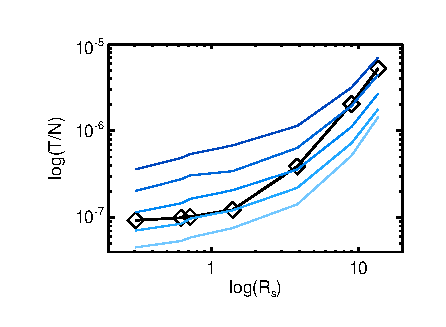
\includegraphics[scale=1.0]{part4/Gheller_P013/P013-2.eps}
\caption{Comparison of GPU and CPU performance at different average radii $R_s$: the black line shows the GPU
computing time per particle. Blue lines show the CPU performance starting from 16 cores (light blue)
to one core (dark blue).}
\label{fig:gpucpu}
\end{figure}

\bibliography{editor}
